\documentclass[tikz,border=3pt]{standalone}
\usepackage[T1]{fontenc}
\usepackage{newtxtext,newtxmath}
\usetikzlibrary{arrows.meta,calc}
\definecolor{ink}{HTML}{23343F}
\definecolor{blue}{HTML}{2276A0}
\definecolor{teal}{HTML}{087F78}
\definecolor{orange}{HTML}{C46B2C}
\definecolor{muted}{HTML}{4C5D67}
\definecolor{rule}{HTML}{D6DFE3}
\begin{document}
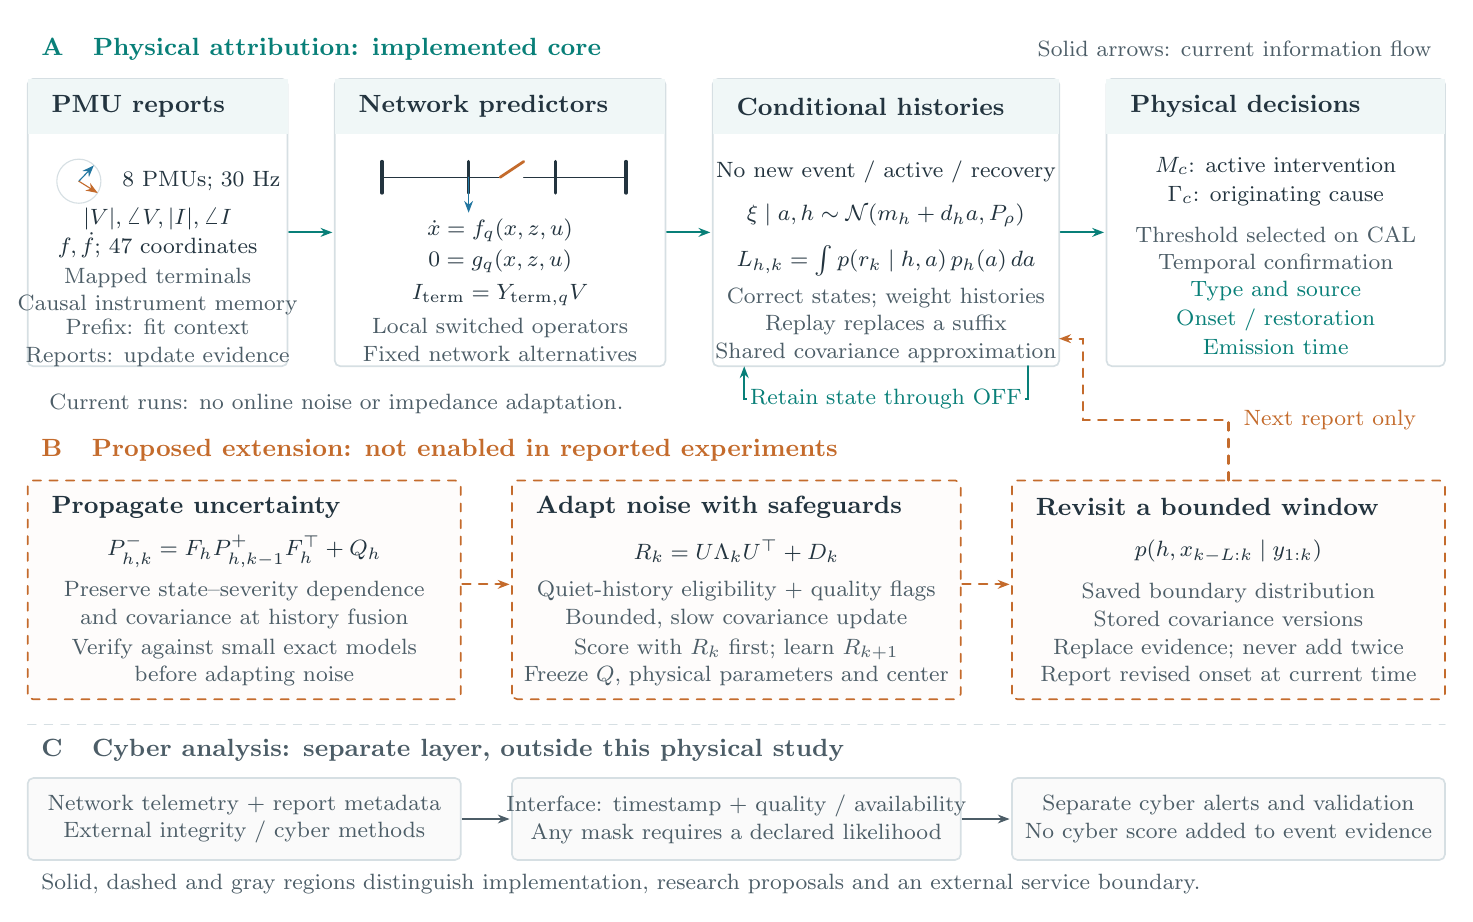
\begin{tikzpicture}[font=\fontsize{8.5}{10.5}\selectfont,text=ink,
 >={Stealth[length=1.5mm]},line cap=round,
 card/.style={draw=rule,rounded corners=2pt,fill=white,line width=.6pt},
 head/.style={font=\bfseries\fontsize{9}{11}\selectfont,anchor=west},
 note/.style={font=\fontsize{8}{10}\selectfont,text=muted},
 flow/.style={->,draw=teal,line width=.8pt},
 proposed/.style={->,draw=orange,dashed,line width=.8pt}]
\path[use as bounding box] (0,0) rectangle (18,11);
\node[head,text=teal] at (.05,10.73) {A\quad Physical attribution: implemented core};
\node[note,anchor=east] at (17.95,10.73) {Solid arrows: current information flow};
\foreach \a/\b in {0/3.3,3.9/8.1,8.7/13.1,13.7/18}{
 \path[card] (\a,6.7) rectangle (\b,10.35);
 \fill[teal!6] (\a,9.65) rectangle (\b,10.35);
}
\node[head] at (.18,10.0) {PMU reports};
\node[head] at (4.08,10.0) {Network predictors};
\node[head] at (8.88,10.0) {Conditional histories};
\node[head] at (13.88,10.0) {Physical decisions};
% Input icon and measurement contract.
\draw[rule] (.65,9.05) circle (.28);
\draw[blue,->] (.65,9.05)--(.84,9.25);
\draw[orange,->] (.65,9.05)--(.89,8.9);
\node[anchor=west] at (1.08,9.05) {8 PMUs; 30 Hz};
\node[align=center] at (1.65,8.40) {$|V|,\angle V,|I|,\angle I$\\$f,\dot f$; 47 coordinates};
\node[note,align=center] at (1.65,7.65) {Mapped terminals\\Causal instrument memory};
\node[note,align=center] at (1.65,7.0) {Prefix: fit context\\Reports: update evidence};
% Physical rather than learned graph: small branch motif.
\foreach \x in {4.5,5.6,6.7,7.6}{\draw[ink,line width=1.2pt] (\x,8.9)--(\x,9.3);}
\draw[ink] (4.5,9.1)--(5.6,9.1)--(6.0,9.1) (6.3,9.1)--(7.6,9.1);
\draw[orange,line width=1pt] (6.0,9.1)--(6.3,9.3);
\draw[blue,->] (5.6,9.1)--(5.6,8.65);
\node at (6.0,8.43) {$\dot x=f_q(x,z,u)$};
\node at (6.0,8.03) {$0=g_q(x,z,u)$};
\node at (6.0,7.60) {$I_{\rm term}=Y_{{\rm term},q}V$};
\node[note,align=center] at (6.0,7.04) {Local switched operators\\Fixed network alternatives};
\node[align=center] at (10.9,9.17) {No new event / active / recovery};
\node at (10.9,8.62) {$\xi\mid a,h\sim\mathcal N(m_h+d_ha,P_\rho)$};
\node at (10.9,8.04) {$L_{h,k}=\int p(r_k\mid h,a)\,p_h(a)\,da$};
\node[note,align=center] at (10.9,7.22) {Correct states; weight histories\\Replay replaces a suffix\\Shared covariance approximation};
\node[align=center] at (15.85,9.05) {$M_c$: active intervention\\$\Gamma_c$: originating cause};
\node[note,align=center] at (15.85,8.17) {Threshold selected on CAL\\Temporal confirmation};
\node[align=center,text=teal] at (15.85,7.32) {Type and source\\Onset / restoration\\Emission time};
\draw[flow] (3.32,8.4)--(3.87,8.4);
\draw[flow] (8.12,8.4)--(8.67,8.4);
\draw[flow] (13.12,8.4)--(13.67,8.4);
\draw[flow] (12.7,6.7)--(12.7,6.28)--(9.1,6.28)--(9.1,6.7);
\node[note,text=teal,fill=white,inner sep=1pt] at (10.9,6.28) {Retain state through OFF};
\node[note,anchor=west] at (.15,6.22) {Current runs: no online noise or impedance adaptation.};

\node[head,text=orange] at (.05,5.63) {B\quad Proposed extension: not enabled in reported experiments};
\foreach \a/\b in {0/5.5,6.15/11.85,12.5/18}{
 \path[card,draw=orange,dashed,fill=orange!2] (\a,2.47) rectangle (\b,5.25);
}
\node[head] at (.18,4.91) {Propagate uncertainty};
\node at (2.75,4.35) {$P^-_{h,k}=F_hP^+_{h,k-1}F_h^\top+Q_h$};
\node[note,align=center] at (2.75,3.67) {Preserve state--severity dependence\\and covariance at history fusion};
\node[note,align=center] at (2.75,2.94) {Verify against small exact models\\before adapting noise};
\node[head] at (6.33,4.91) {Adapt noise with safeguards};
\node at (9.0,4.35) {$R_k=U\Lambda_kU^\top+D_k$};
\node[note,align=center] at (9.0,3.67) {Quiet-history eligibility + quality flags\\Bounded, slow covariance update};
\node[note,align=center] at (9.0,2.94) {Score with $R_k$ first; learn $R_{k+1}$\\Freeze $Q$, physical parameters and center};
\node[head] at (12.68,4.91) {Revisit a bounded window};
\node at (15.25,4.35) {$p(h,x_{k-L:k}\mid y_{1:k})$};
\node[note,align=center] at (15.25,3.67) {Saved boundary distribution\\Stored covariance versions};
\node[note,align=center] at (15.25,2.94) {Replace evidence; never add twice\\Report revised onset at current time};
\draw[proposed] (5.52,3.93)--(6.12,3.93);
\draw[proposed] (11.87,3.93)--(12.47,3.93);
\draw[proposed] (15.25,5.25)--(15.25,6.02)--(13.4,6.02)--(13.4,7.05)--(13.1,7.05);
\node[note,text=orange,anchor=west,fill=white,inner sep=1pt] at (15.4,6.02) {Next report only};

% Separate service boundary: no attack score is a physical likelihood.
\draw[rule,dashed] (0,2.15)--(18,2.15);
\node[head,text=muted] at (.05,1.82) {C\quad Cyber analysis: separate layer, outside this physical study};
\path[card,fill=black!2] (0,.43) rectangle (5.5,1.47);
\path[card,fill=black!2] (6.15,.43) rectangle (11.85,1.47);
\path[card,fill=black!2] (12.5,.43) rectangle (18,1.47);
\node[note,align=center] at (2.75,.95) {Network telemetry + report metadata\\External integrity / cyber methods};
\node[note,align=center] at (9,.95) {Interface: timestamp + quality / availability\\Any mask requires a declared likelihood};
\node[note,align=center] at (15.25,.95) {Separate cyber alerts and validation\\No cyber score added to event evidence};
\draw[->,muted] (5.52,.95)--(6.12,.95);
\draw[->,muted] (11.87,.95)--(12.47,.95);
\node[note,anchor=west] at (.05,.12) {Solid, dashed and gray regions distinguish implementation, research proposals and an external service boundary.};
\end{tikzpicture}
\end{document}
